\chapter{Einführung}
In unserer vernetzten Welt haben erdnahe Satelliten eine immer größere Bedeutung in der globalen Infrastruktur. Sie finden vor allem Anwendung in der Kommunikation und Erdbeobachtung. Satelliten im nahen Erdorbit (\textit{low earth orbit}, LEO) haben den Vorteil, dass sie deutlich geringere Signallaufzeiten gegenüber geostationären Satelliten aufweisen. Das ermöglicht schnellere Kommunikation. Auch die Aufnahme hochauflösender Messungen der Erdoberfläche wird durch die Flughöhe begünstigt und ist in einer höheren Wiederholrate aufgrund der kürzeren Umlaufdauer möglich. Für den Einsatz im LEO werden immer mehr kleine, kostengünstige Satelliten produziert. Vor allem durch die Kommerzialisierung der Raumfahrtbranche, die im letzten Jahrzehnt durch Unternehmen wie SpaceX und Blue Origin vorangetrieben wurde, sind die Kosten für den Start von Satelliten gesunken und die Zahl der Starts enorm gestiegen. Jeder dieser Satelliten benötigt eine Lageregelung und damit ein Antriebssystem, welches kostengünstig im LEO über lange Zeiten dem atmosphärischen Widerstand entgegenwirken kann.

Damit sind elektrische Antriebssysteme in den Vordergrund gerückt, da sie eine einzigartige und momentan einzig realisierbare Lösung für die lange Betriebsdauer kleiner Satelliten im LEO darstellen. Das liegt an ihrem hohen spezifischem Impuls, der nicht durch die Verwendung chemischer Antriebe erreicht werden kann. Der spezifische Impuls beschreibt wie viel Impulsänderung pro ausgestoßene Masse erreicht werden kann und ist damit von der Austrittsgeschwindigkeit des Treibstoffes bestimmt. Der hohe spezifische Impuls elektrischer Triebwerke ist im Wesentlichen darauf zurückzuführen, dass die für die Beschleunigung eingesetzte Energie nicht aus dem Treibstoff selbst kommt, wie es bei chemischen Triebwerken der Fall ist, sondern über ein elektrisches Feld von außen eingespeist wird. Damit sind elektrische Antriebe effizienter und können mit weniger Treibstoff mehr Impulsänderung erreichen, indem sie elektrische Energie aus, zum Beispiel, Solarzellen verwenden. Ein Blick auf die von William Moore und Konstantin Ziolkowski formulierte Raktengleichung
\begin{equation}
    \Delta v = v_e \cdot \ln\left(\frac{m_0}{m_f}\right),
\end{equation}
welche die gesamte erreichbare Änderung der Geschwindigkeit $\Delta v$ beschreibt, veranschaulicht die Abhängigkeit von der Austrittsgeschwindigkeit $v_e$, während das Masseverhätnis $\frac{m_0}{m_f}$ nur logarithmisch eingeht.

Eines dieser elektrischen Antriebssysteme ist das Radiofrequenzionentriebwerk (RIT). Es wurde von Prof. Löb an der Justus Liebig Universität (JLU) Gießen in den 60er Jahren entwickelt und steht auch heute noch im Fokus der Forschung an der JLU, weshalb es in dieser Arbeit besonders von Relevanz ist. Das RIT ist neben dem Hall-Effekt-Thruster (HET) eines der effizientesten elektrischen Triebwerke und wurde bereits auf mehreren erfolgreichen Missionen eingesetzt \cite[S. 6]{ion}. Die BepiColombo-Mission 2018 ist ein bekanntes Beispiel.

Das RIT ist ein sogenanntes Gitterionentriebwerk, welches auf der Ionisierung von Gasen basiert, welche dann elektrostatisch auf sehr hohe Austrittsgeschwindigkeiten beschleunigt werden. Dafür wird im Triebwerk ein Plasma gezündet, in dem über magnetische Wecheslfelder Energie auf freie Elektronen übertragen wird, die dann, Stoßionisationen durchführen können. Der historisch am häufigsten verwendete Treibstoff für das RIT ist Xenon. Xenon hat eine hohe Masse und ist ein reaktions-träges Edelgas. Es hat sich bereits bei eine Vielzahl von Missionen bewährt. Nachteilhaft ist allerdings, das die Gewinnung von Xenon äußert aufwendig ist. Sie basiert ausschließlich auf der Luftrennung und anschließenden Extraktion aus flüssigem Sauerstoff. Das macht Xenon zu einem sehr teuren Treibstoff, dessen Produktion nicht dem steigenden Bedarf nachkommen kann. Auch zu beachten, ist sein enormer Energiebedarf und damit verbundener hoher CO$_2$-Faktor von etwa 500 \cite{CO2}. Deswegen hat in den letzten Jahren die Forschung an alternativen Treibstoffen für elektrische Antriebe stark an Relevanz gewonnen. Alternative Treibstoffe sind vorallem für den Einsatz auf kleinen, kommerziellen Satelliten interessant. 

Herauszufinden, ob ein Treibstoff geeignet ist, ist allerdings nicht trivial. Es müssen viele Faktoren berücksichtigt werden, die sowohl mit den Eigenschaften des Treibstoffs selbst, mit den Prozessen bei der Ionisation als auch der Interaktion des Treibstoffs und Triebwerks zusammenhängen. Bevor extensive Tests mit dem Triebwerk direkt durchgeführt werden, kann die Untersuchung der Ionisationseigenschaften und Querschnitte bereits viele wichtige Informationen gewinnen und so Kandidaten früh ausschließen und Vorhersagen über die Effizienz treffen. Sehr wichtige Größen sind dabei die Ionisationsenergie, der Ionisationswirkungsquerschnitt, die Ionisationsrate und die Häufigkeitsverteilung der verschiedenen Ionen, die bei der Ionisation entstehen \cite{ion}. Diese Größen sind besonders für die Beschreibung des Plasmas und somit auch für die Optimierung des Antriebs entscheidend. 

\section{Zielsetzung}
In dieser Arbeit soll es darum gehen, die Elektronenstoßionisation und die daraus entstehenden Produkte verschiedener Gase experimentell zu charakterisieren und somit ihre Nutzbarkeit als Treibstoff für ein RIT zu bewerten. Dafür sollen in Kapitel \ref{chap:ion} die physikalischen Grundlagen der Elektronenstoßionisation und die Ansätze für theoretische Beschreibungen der verschiedenen Ionisationsprozesse diskutiert werden.

Die Ionisation des Treibstoffs und dessen Beschleunigung können in der Regel als voneinander getrennte Prozesse betrachtet werden \cite{ion}. Um das Verhalten eines Gases, und somit auch seine Effizienz als Treibgas, in einem RIT zu bewerten, ist es wichtig das im Entladungsgefäß gezündete Plasma möglichst gut zu verstehen. Die oben genannten, für die Effizienz des Antriebs relevanten Größen, sollen in dieser Arbeit experimentell bestimmt werden. GASE aufzählen

\section{Methodik} 
Die Ionisation wird dabei nicht in einem RIT durchgeführt, sondern in einer Elektronenstoßionisationsanlage. Da primär die Massenspektren und Wirkungsquerschnitte von Relevanz sind, kann die Testanlage so deutlich simpler gestaltet werden und es wird kein Radiofrequenzgenerator benötigt. Basierend auf früheren Arbeiten der Arbeitsgruppe für Ionentriebwerke an der JLU, wird in dieser Arbeit eine bestehen Anlage zur Elektronenstoßionisation ausgebaut. Für das Messen der relevanten Größen müssen die Ionen nachgewiesen und identifiziert werden können. Dafür soll zunächst ein neuer Detektor installiert werden, der eine höhere Auflösung und einen größeren Durchmesser aufweist. Mithilfe des Detektors kann der Zeitpunkt des Auftreffens und der Ort einzelner Ionen bestimmt. Damit die Ionen konsistent auf den Detektor treffen, werden sie mit einem elektrischen Feld beschleunigt und ihre Flugzeit gemessen. Der Aufbau der Anlage ähnelt dem von Straub et al. aus \cite{Straub}, der bereits in den 90er-Jahren viele Flugzeitspektren und Wirkungsquerschnitte mittels Elektronenstoßionisationen aufgenommen hat. Seine Messungen werden auch als Referenz für die ersten Aufnahmen mit Argon in dieser Arbeit dienen, um die Funktionsfähigkeit der Anlage zu überprüfen.

Eine Flugzeitmessung ist eine der zentralen Methoden in der Massenspektroskopie. Sie basiert darauf die Flugzeit einzelner zuvor beschleunigter Teilchen für eine bestimmte Strecke im Vakuum zu messen. In dieser Arbeit wird über eine Flugzeitmessung das Masse-zu-Ladungsverhältnis einzelner Ionen bestimmt. Im Folgenden wird gezeigt, wie die Geschwindigkeit und Flugzeit von Ionen einen Rückschluss auf ihre Masse und Ladung geben.

Durch Anlegen eines elektrischen Feldes, können elektrisch geladene Teilchen über die Coulombkraft beschleunigt werden. Die Beschleunigung $a$ welche Ionen mit der Ladung $q_i$ und Masse $m_i$ erfahren, wenn sie sich in einem elektrischen Feld mit der Feldstärke $E$ befinden wird in Formel \ref{eq:beschleunigung} beschrieben: 
\begin{equation}
    \label{eq:beschleunigung}
    a = \frac{q_i}{m_i} \cdot E.
\end{equation}
Die Flugzeit $t_f$ der Ionen über einer festen Strecke $d$ im Feld kann dann wie folgt beschrieben werden.
\begin{equation}
    t_f = \sqrt{\frac{m_i}{q_i}} \cdot \sqrt{\frac{2d}{E}} = \sqrt{\frac{m_i}{q_i}} \cdot \sqrt{\frac{2}{U}} \cdot d
\end{equation}
Hieraus ist offensichtlich, dass eine Variation der Flugzeit allein von ihrem Masse-zu-Ladungsverhältnis $\frac{m_i}{q_i}$ abhängt, wenn die Spannung $U$ und der Abstand $d$ konstant bleiben. Treten die Ionen aus dem Feld aus fliegen sie weiter mit konstanter Geschwindigkeit unabhängig ihrer Eigenschaften. Ein Flugzeitspektrum zeigt dann höher geladene Ionen desselben Elements mit einer geringeren Flugzeit. In der Theorie ist dises Spektrum diskret für verschiedene Masse zu Ladungsverhältnisse, im Labor sind die Peaks jedoch etwas ausgedehnt, wie in Abbildung \ref{fig:rest_tof} zu sehen. Das liegt daran, dass die Flugzeit und der Ort der Entstehung der Teilchen nicht genau gemessen werden können. In Abbildung \ref{fig:rest} sieht man ein Masse-zu-Ladungsspektrum der Restgase in der Vakuumkammer. 

Um die Flugzeit experimentell zu bestimmen, wird ein Start- und Stoppsignal benötigt. Der Startzeitpunkt muss den Eintritt in das elektrische Feld markieren und der Stoppzeitpunkt das Auftreffen auf einen Detektor. Kritisch ist dabei, die Flugzeit mit hinreichender Genauigkeit unabhängig vom Ion zu bestimmen. Typische Flugzeiten sind in diesem Aufbau in der Größenordnung von Mikrosekunden. Wie auch in der Arbeit von Straub et al. wird ein Pulsgenerator verwendet, der einen Hochspannungspuls auf einer Ablenkplatte, und damit das elektrische Feld zur Beschleunigung der Ionen erzeugt. Der Puls, der diese Spannung triggert wird auch als Startsignal verwendet.

\begin{figure}
    \centering
    \hspace*{-.8cm}
    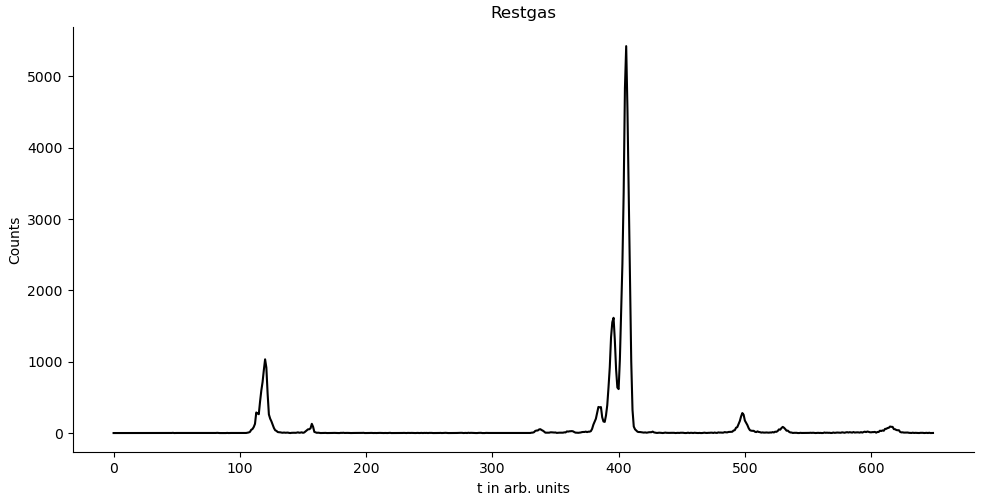
\includegraphics[width=.95\textwidth]{Restgas_tof.png}
    \caption[Flugzeitspektrum der Restgase]{Unskaliertes Flugzeitspektrum der Restgase in der Vakuumkammer. Die Zeitachse ist in willkürlichen Einheiten angegeben. Zur Bestimmung der Masse-zu-Ladungsverhältnisse muss das Spektrum anhand einiger Annahmen skaliert werden.}
    \label{fig:rest_tof}
\end{figure}

\begin{figure}
    \centering
    \hspace*{-1cm}
    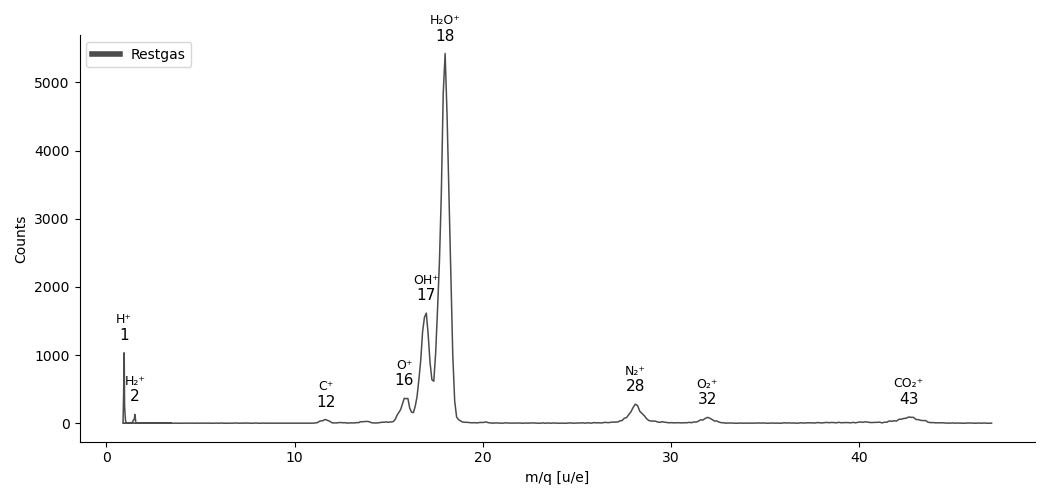
\includegraphics[width=1.05\textwidth]{Restgas.png}
    \caption[Masse-zu-Ladungsspektrum der Restgase]{Masse-zu-Ladungsspektrum der Restgase erzeugt aus dem Flugzeitspektrum in Abb. \ref{fig:rest_tof}. Die Peaks entsprechen den verschiedenen Ionen, die durch die Elektronenstoßionisation entstanden sind. Für die Identifikation der Ionen wurde angenommen, das der größte Peak ionisierten Wassermolekülen entspricht und der erste Peak ionisiertem Wasserstoff. Dadurch konnte das Spektrum skaliert werden und die Masse zu Ladungsverhältnisse der anderen Ionen bestimmt werden.}
    \label{fig:rest}
\end{figure}